\begin{frame}{Balance del GNC con y sin ajuste de causación del FEPC}

\begin{figure}
\centering
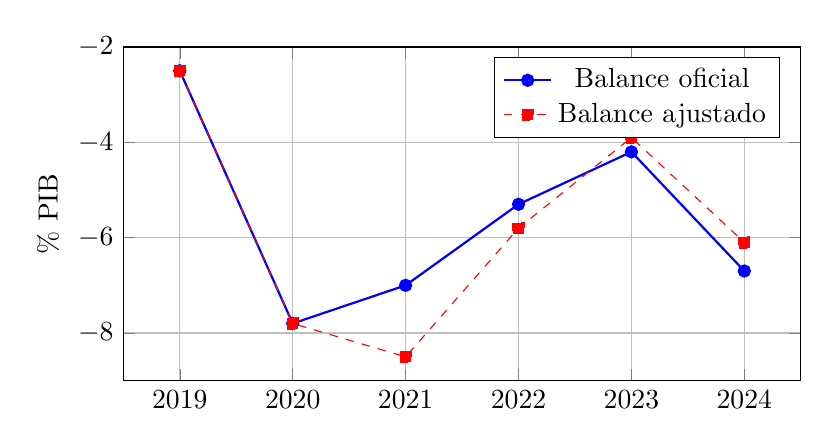
\begin{tikzpicture}
\begin{axis}[
    width=0.84\textwidth, height=0.48\textwidth,
    ylabel={\% PIB},
    symbolic x coords={2019, 2020, 2021, 2022, 2023, 2024},
    xtick=data,
    ymin=-9, ymax=-2,
    legend pos=north east,
    grid=both,
    minor grid style={dotted},
    major grid style={solid},
    ylabel near ticks,
    xlabel near ticks
]

% Datos del déficit oficial
\addplot[
    color=blue,
    mark=*,
    thick
] coordinates {
    (2019, -2.5)
    (2020, -7.8)
    (2021, -7.0)
    (2022, -5.3)
    (2023, -4.2)
    (2024, -6.7)
};
\addlegendentry{Balance oficial}

% Datos del déficit ajustado
\addplot[
    color=red,
    mark=square*,
    dashed
] coordinates {
    (2019, -2.5)
    (2020, -7.8)
    (2021, -8.5)
    (2022, -5.8)
    (2023, -3.9)
    (2024, -6.1)
};
\addlegendentry{Balance ajustado}

\end{axis}
\end{tikzpicture}

\vspace{0.1cm}
\scriptsize\textit{Fuente: elaboración propia con base en el Balance Fiscal del GNC, MHCP. El MFMP 2026 no publica el balance 2025 con el mismo ajuste de causación.}
\end{figure}

\end{frame}
